\documentclass[12pt,preprint]{aastex}
\usepackage{geometry,amsmath}
\usepackage{float}
%\usepackage{titlesec} %used to format titles
\usepackage{graphicx} %for handling figures
\usepackage[none]{hyphenat} %disallows hyphenated words


\begin{document}

\title{HERA Dish Reflectometry} 
\author{Zaki Ali, Carina Cheng, Aaron Parsons, Nipanjana Patra}
\maketitle

\section{Introduction}

There are several different sources of instrumental chromaticity for an interferometer such as HERA that each introduce unwanted systematics in data. One such source results from the antenna, which can introduce non-spectrally smooth structure in data due to delays associated with internal signal reflections. The HERA element was designed to minimize this structure - the contamination outside the foreground `wedge' - so that the expected level of the 21cm reionization signal that we are interested in still dominates this region. In order to achieve this, a chromaticity specification of -60 dB at 60 ns was implemented in the HERA element design, setting a constraint on the level of reflections. In other words, when a signal that originates at the feed re-enters the feed after a time delay of 60 ns, it must be attenuated by at least 60 dB. 

Understanding the nature of antenna reflections in the HERA dish is of the utmost importance in characterizing the performance of the dish. As HERA progresses as an experiment, it is necessary to build optimal dishes that promise to minimize the challenges of chromaticity in our quest for the Epoch of Reioinization.

\section{Set-Up}

To measure the delays associated with reflections within the dish and feed, we
used the prototype HERA dish (Figure \ref{fig:heradish} built at the NRAO site in
Green Bank, WV. The dish is a 14-m parabolic reflector structurally supported
with 3 telephone poles. The reflective material is made up of wire mesh that
is attached to the PVC pipes that form the parabolic shape. With the current
prototype, the feed is a PAPER dipole encased in a cylindrical cage encompassing
the backplane. The PAPER feed and the backplane (which prevents feed-to-feed
interaction between neighboring dishes) is raised and lowered by a three pulley
system. The focal height of the dish is 4.5 m ($sim{14.76}$).

The following reflectometry measurements were taken on July 20-23, 2015 using a
FieldFox unit in Network Analyzer mode. A pulse was generated in the FieldFox
and sent through a 75ft $50\Omega$ cable that connected to the feed with a 4:1
passive balun. This signal gets transmitted through the feed and then reflects
off the dish...



\begin{figure}
\centering
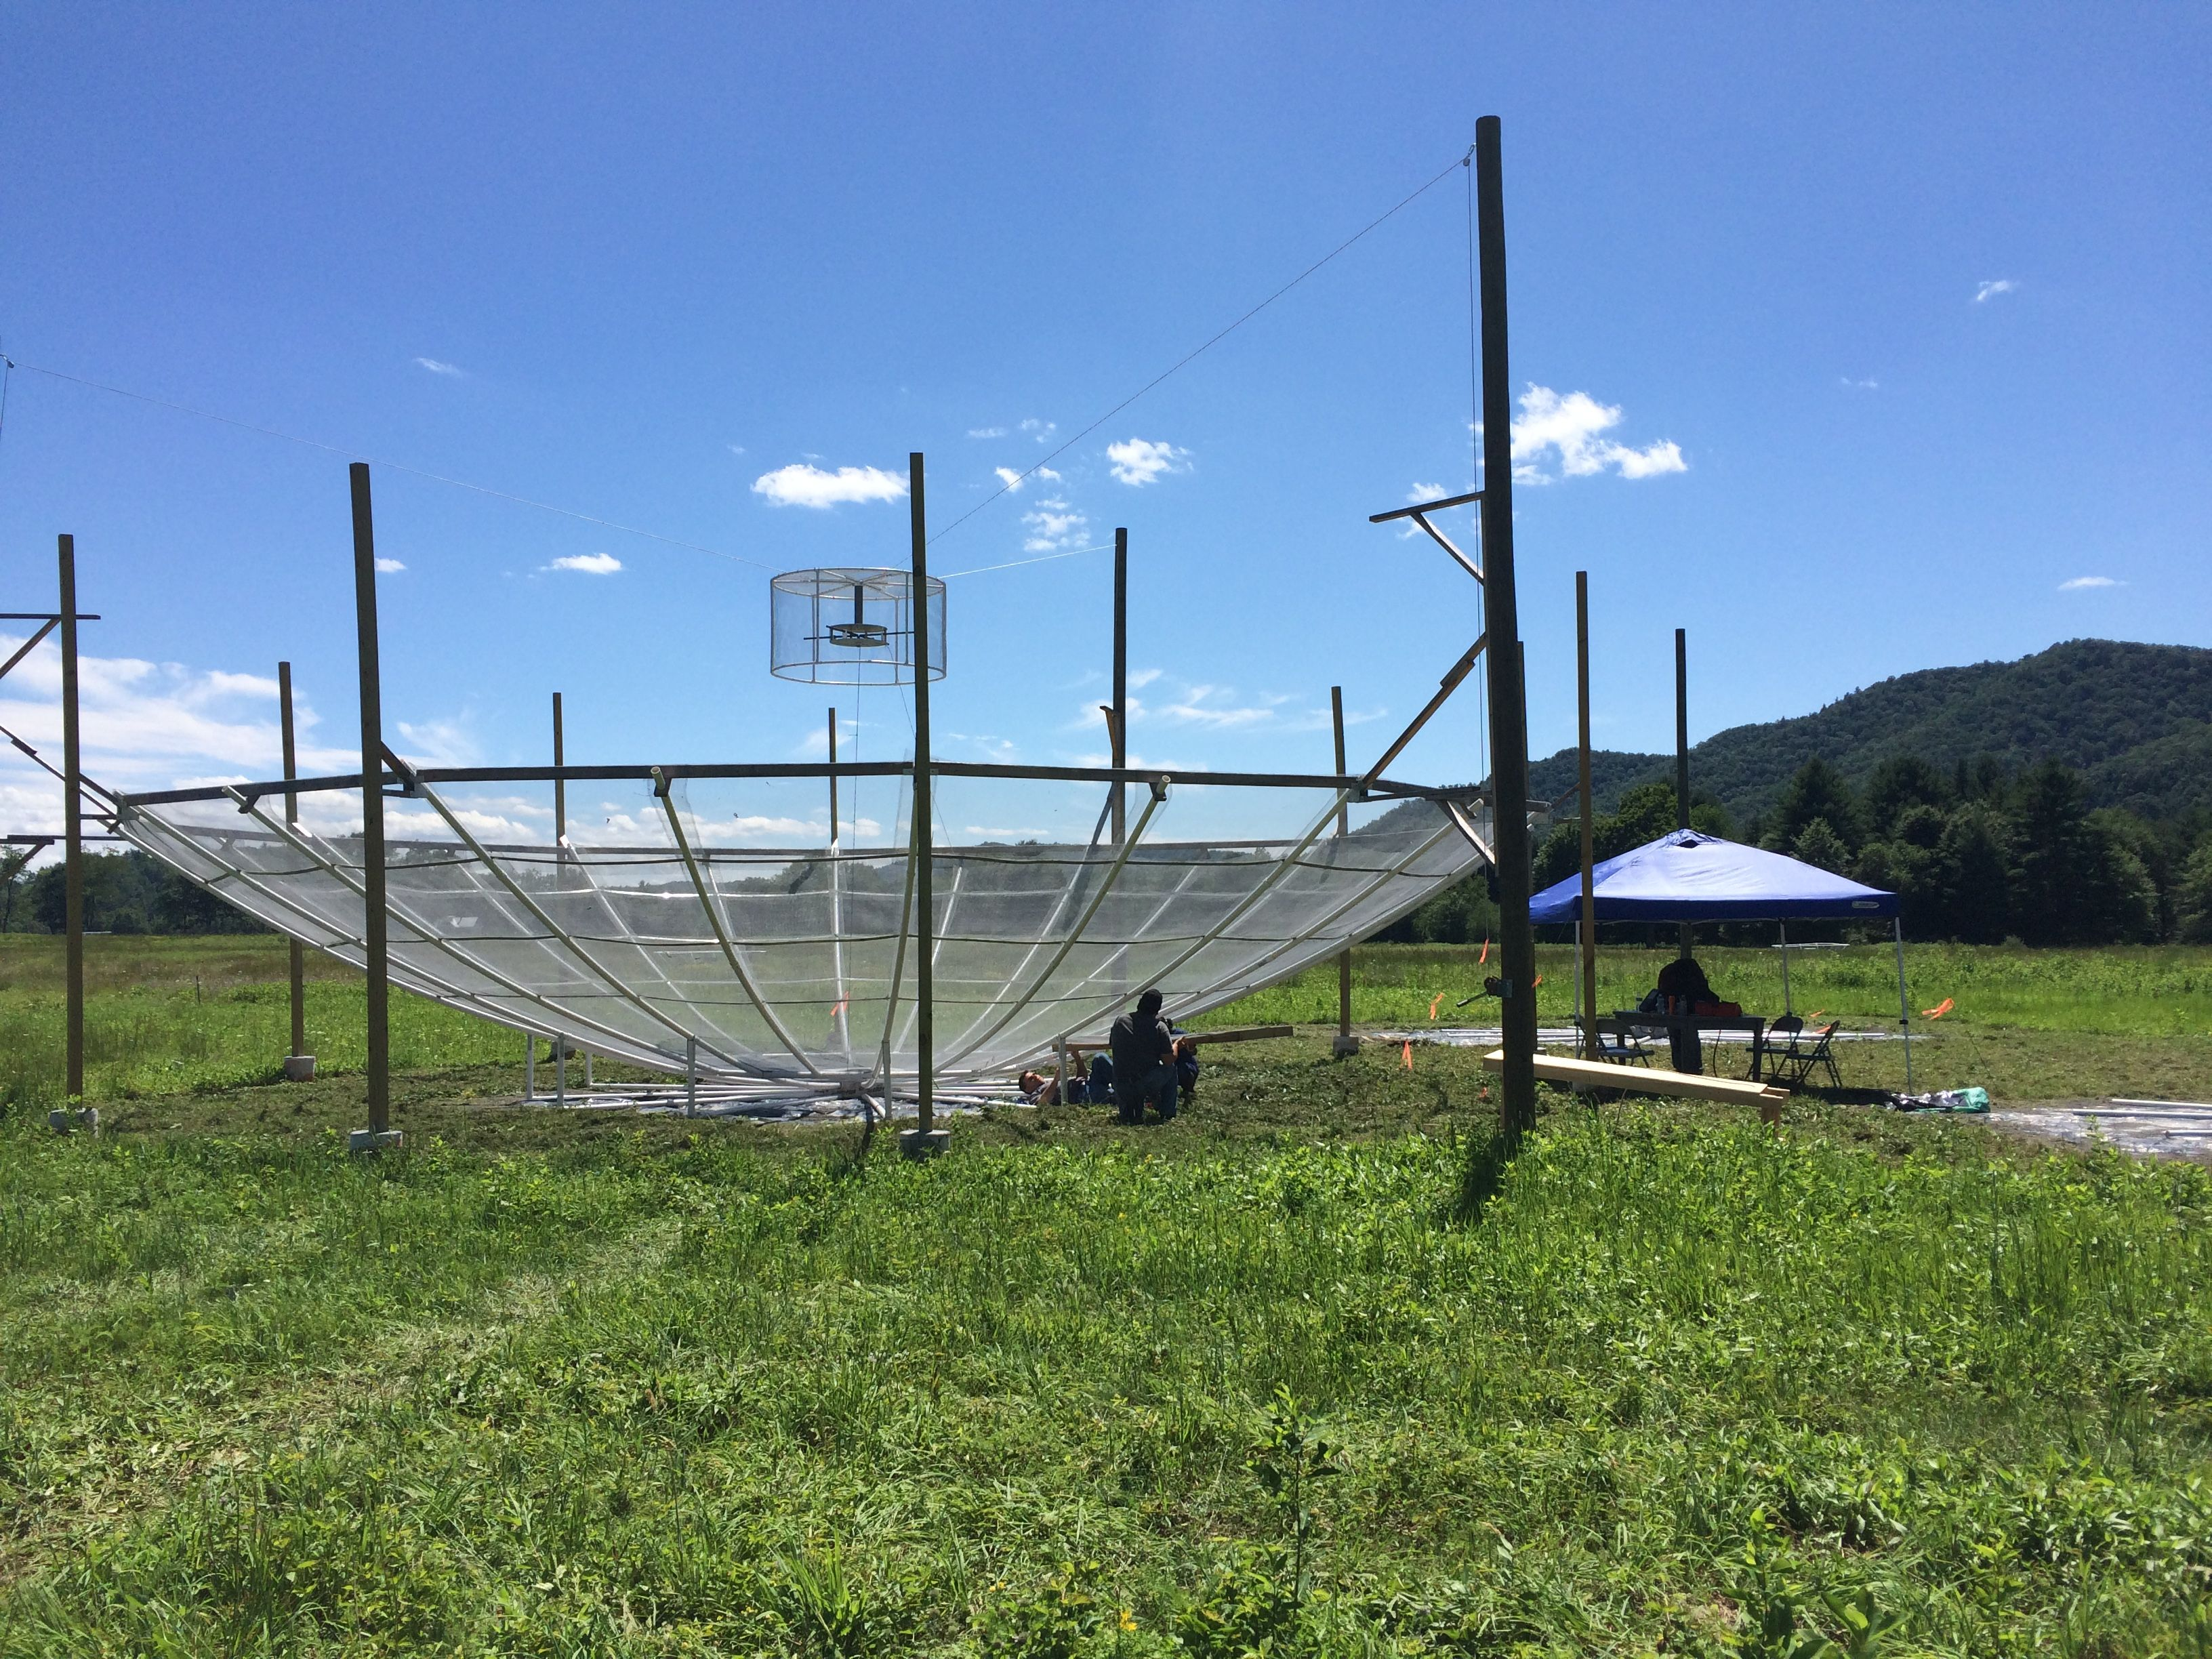
\includegraphics[trim={2cm 20cm 30cm 15cm},clip, totalheight=0.45\textheight]{plots/heradish.jpg}
\caption{HERA dish and feed at the Green Bank NRAO site.}
\label{fig:heradish}
\end{figure}

\section{Theory}

*what is the measurement we are actually doing. 

*compare cable pulse measurements vs. actual sky measurements and how the amount of signal that is transmitted/reflected is different*

*explain why the level of the measurements has to be brought down, and how this is okay for high delays*

\begin{figure}
\centering
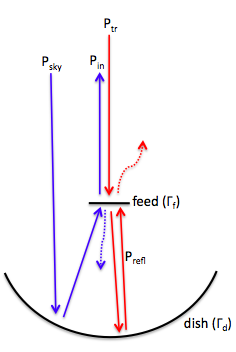
\includegraphics[totalheight=0.5\textheight]{plots/reflection_cartoon.png}
\caption{The blue solid lines represent an original sky signal entering the feed. A small percentage of it (dashed blue) is reflected off the dish, and it is these reflections that we are concerned about. In our measurements however, the reflections measured contain most of the original pulse signal (solid red), so it is crucial to adjust for this difference in our analysis.}
\end{figure}


\section{Measurements}

We begin with a reflectometry measurement with the feed suspended at 12 ft (distance between the balun and top of the central hub) for a frequency bandwidth of 50MHz - 500MHz.

\begin{figure}
\centering
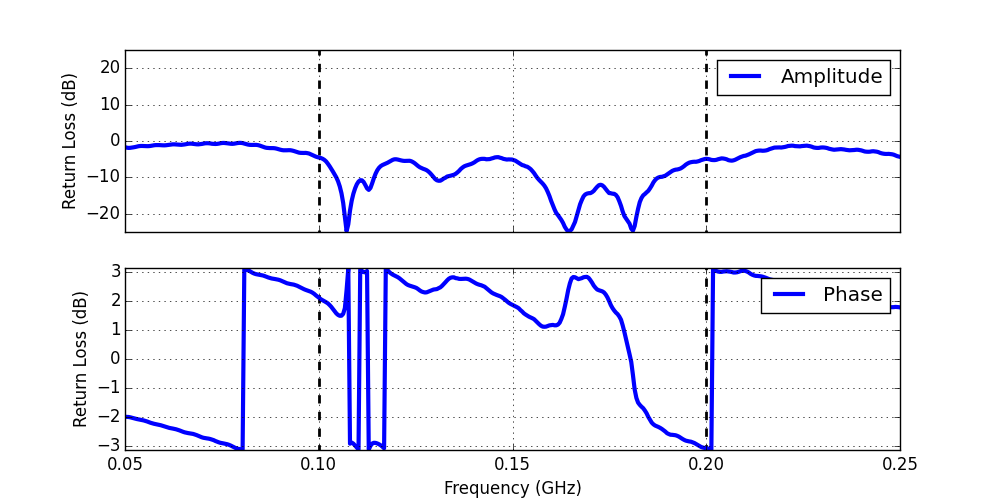
\includegraphics[totalheight=0.4\textheight]{plots/frequency_amp_phase.png}
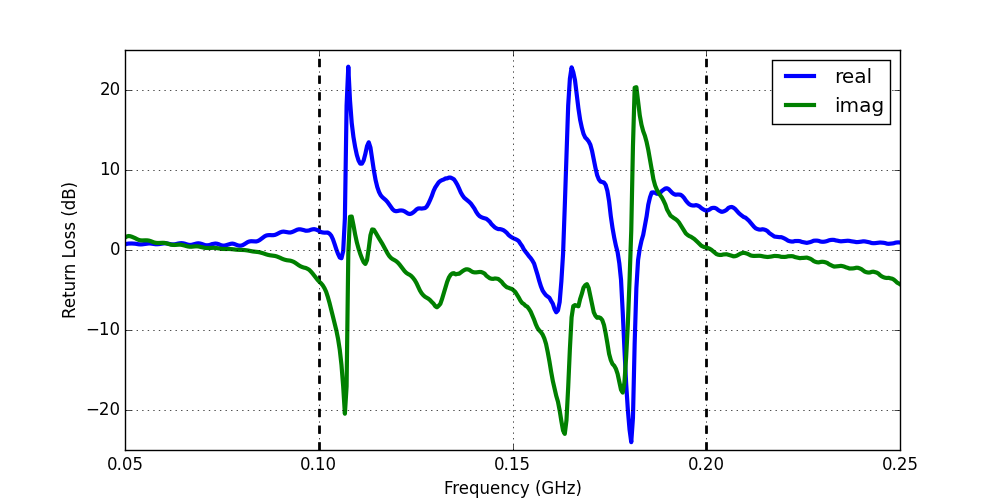
\includegraphics[totalheight=0.4\textheight]{plots/frequency_real_imag.png}
\caption{Top: Amplitude and phase of the reflected signal. Bottom: Real part and imaginary part of the reflected signal.}
\end{figure}

Next, we Fourier-transform along the frequency axis for 3 selected bandwidths: 50MHz-250MHz (the HERA bandwidth), 100MHz-200MHz (the PAPER bandwidth), and 140MHz-160MHz (bandwidth particularly relevant for making power spectra). This produces delay plots that shows...

\begin{figure}
\centering
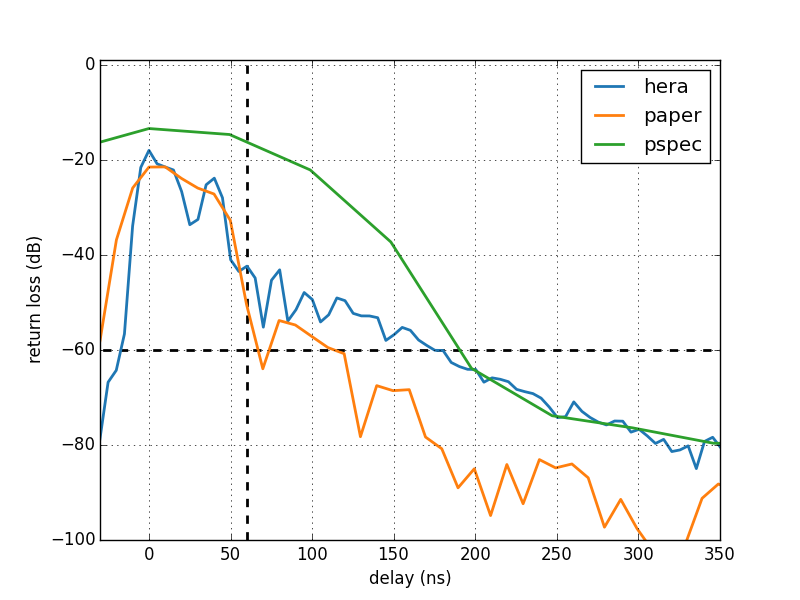
\includegraphics[totalheight=0.5\textheight]{plots/delay3_window.png}
\caption{Delay plots produced using a Blackman-Harris window function for 3 different frequency bandwidths.}
\end{figure}

The importance of window functioning when Fourier-transforming is illustrated in Figure...

\begin{figure}
\centering
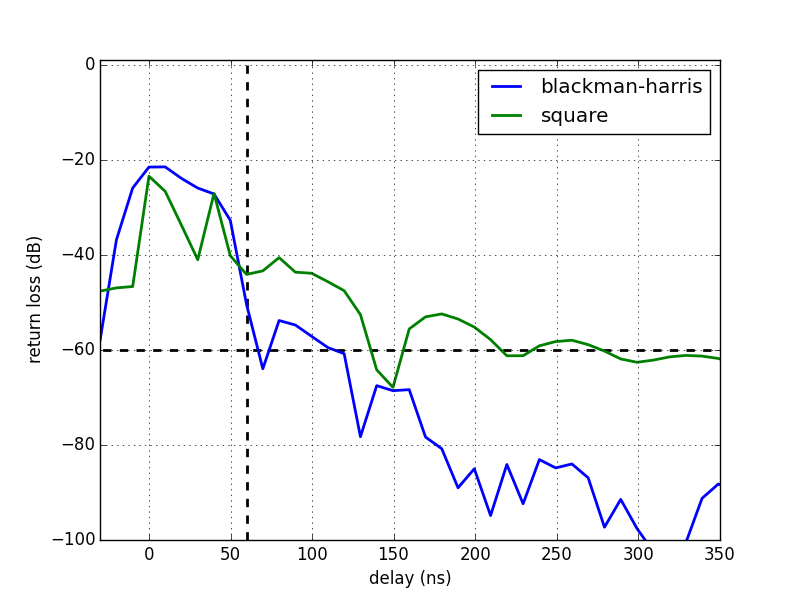
\includegraphics[totalheight=0.5\textheight]{plots/bh_vs_sq.png}
\caption{Delay plot produced using a Blackman-Harris window function vs. a square window function for the PAPER bandwidth.}
\end{figure}

Finally, more robust measurements are taken with the feed at varying heights (6ft, 9ft, 12ft, and 15ft)...

\begin{figure}
\centering
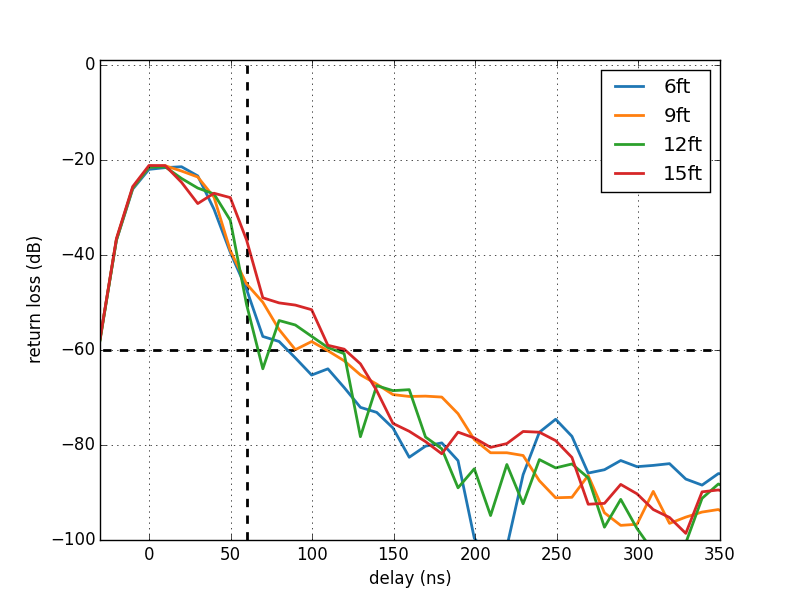
\includegraphics[totalheight=0.5\textheight]{plots/delay_heights_paper.png}
\caption{Delay plots produced using a Blackman-Harris window function for 4 different feed heights and the PAPER bandwidth.}
\end{figure}

\begin{figure}
\centering
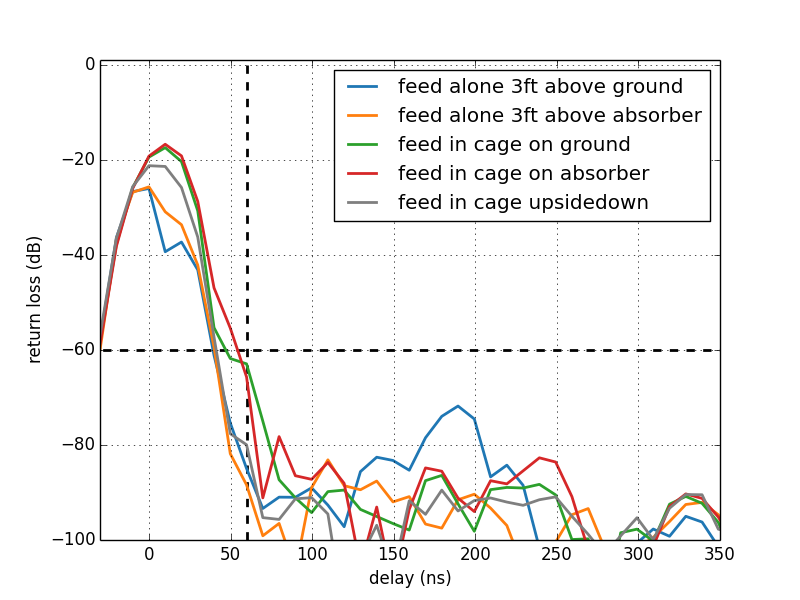
\includegraphics[totalheight=0.5\textheight]{plots/delay_feed.png}
\caption{Delay plots produced using a Blackman-Harris window function for different lone feed configurations and the PAPER bandwidth.}
\end{figure}


\section{Discussion}

\section{Conclusion}


\end{document}
